\documentclass[10pt,a4paper]{article}
\usepackage[margin=1.4cm]{geometry}
\usepackage{multicol}
\usepackage[T1]{fontenc}
\usepackage[utf8]{inputenc}
\usepackage{amsmath,amssymb,amsthm,mathtools}
\usepackage{xcolor}
\usepackage[most]{tcolorbox}
\usepackage{enumitem}
\usepackage{booktabs}
\usepackage{array}
\usepackage{graphicx}
\usepackage{caption}
\usepackage{float}
\usepackage[colorlinks=true,linkcolor=teal,urlcolor=blue,citecolor=teal]{hyperref}

\definecolor{cQ}{HTML}{1F4E79}      \definecolor{cQBg}{HTML}{F0F5FA}
\definecolor{cKey}{HTML}{1B5E20}    \definecolor{cKeyBg}{HTML}{E8F5E9}
\definecolor{cTrap}{HTML}{B71C1C}   \definecolor{cTrapBg}{HTML}{FFEBEE}
\definecolor{cWhy}{HTML}{4A148C}    \definecolor{cWhyBg}{HTML}{F3E5F5}
\definecolor{cThm}{HTML}{E65100}    \definecolor{cThmBg}{HTML}{FFF3E0}
\definecolor{cNew}{HTML}{AD1457}    \definecolor{cNewBg}{HTML}{FCE4EC}
\definecolor{cSay}{HTML}{01579B}    \definecolor{cSayBg}{HTML}{E1F5FE}
\definecolor{cNote}{HTML}{616161}

\newtcolorbox{keybox}[1][]{breakable,enhanced,colback=cKeyBg,colframe=cKey,
  boxrule=1pt,left=5pt,right=5pt,top=4pt,bottom=4pt,arc=2pt,
  fonttitle=\bfseries\sffamily,coltitle=black,title={#1}}
\newtcolorbox{whybox}[1][]{breakable,enhanced,colback=cWhyBg,colframe=cWhy,
  boxrule=0.8pt,left=5pt,right=5pt,top=4pt,bottom=4pt,arc=2pt,
  fonttitle=\bfseries\sffamily,title={#1}}
\newtcolorbox{thmbox}[1][]{breakable,enhanced,colback=cThmBg,colframe=cThm,
  boxrule=1pt,left=5pt,right=5pt,top=4pt,bottom=4pt,arc=2pt,
  fonttitle=\bfseries\sffamily,coltitle=black,title={#1}}
\newtcolorbox{trapbox}[1][]{breakable,enhanced,colback=cTrapBg,colframe=cTrap,
  boxrule=0.7pt,left=5pt,right=5pt,top=4pt,bottom=4pt,arc=2pt,
  fonttitle=\bfseries\sffamily,title={#1}}
\newtcolorbox{freshbox}[1][]{breakable,enhanced,colback=cNewBg,colframe=cNew,
  boxrule=1pt,left=5pt,right=5pt,top=4pt,bottom=4pt,arc=2pt,
  fonttitle=\bfseries\sffamily,coltitle=black,title={#1}}
\newtcolorbox{saybox}[1][Say this]{breakable,enhanced,colback=cSayBg,colframe=cSay,
  boxrule=0.8pt,left=5pt,right=5pt,top=4pt,bottom=4pt,arc=2pt,
  fonttitle=\bfseries\sffamily,title={#1}}
\newtcolorbox{qabox}[1][]{breakable,enhanced,colback=cQBg,colframe=cQ,
  boxrule=0.7pt,left=5pt,right=5pt,top=4pt,bottom=4pt,arc=2pt,
  fonttitle=\bfseries\sffamily,title={#1}}

\newcommand{\dd}{\mathrm{d}}
\newcommand{\E}{\mathbb{E}}
\newcommand{\PP}{\mathbb{P}}
\newcommand{\QQ}{\mathbb{Q}}
\newcommand{\F}{\mathcal{F}}
\newcommand{\half}{\tfrac{1}{2}}
\newcommand{\si}{\sigma_{\mathrm{imp}}}
\newcommand{\sr}{\sigma_{\mathrm{real}}}
\captionsetup{font=small,labelfont=bf}

% allow more floats per page; the default 2-top/3-total forces an extra page
\setcounter{topnumber}{3}\setcounter{bottomnumber}{2}\setcounter{totalnumber}{4}
\renewcommand{\topfraction}{0.92}\renewcommand{\bottomfraction}{0.6}
\renewcommand{\textfraction}{0.06}\renewcommand{\floatpagefraction}{0.75}
\setlength{\parindent}{0pt}
\setlength{\parskip}{0.14em}

\title{\vspace{-2.7cm}\textbf{Volatility as a quadratic variation:\\
measuring it, forecasting it, and pricing it on the NIFTY~50}}
\author{%
\small Jaivin Bengani (2024ADPS0850G) \textbullet\ Purunjay Karwa (2024ADPS0857G)\\
\small Soham Agrawal (2024ADPS0829G) \textbullet\ Vrishank Bimlesh Rao (2024ADPS0871G)\\[2pt]
MAC F244 --- Stochastic Calculus and Applications to Finance\\
\small Instructor: Prof.\ Mayank Goel \textbullet\ BITS Pilani, K.\ K.\ Birla Goa Campus}
\date{15 November 2026}

\begin{document}
\maketitle
\vspace{-0.85cm}

\begin{abstract}\small
\noindent
In It\^o calculus volatility is not a parameter fitted to data: it is the quadratic variation
of the log price, $[\log S]_T=\int_0^T\sigma_t^2\dd t$. This project establishes that the
identity makes volatility a \emph{measurable} path functional, and carries it through to a
quantitative consequence. The measurement is first verified where the answer is known: with
$\sigma(t)$ time-varying and specified in advance, realised variance converges to integrated
variance at log--log slope $-0.4986$ against the predicted $-1/2$, its dispersion matching the
closed form $\sqrt{(2T/n)\!\int\!\sigma_t^4\dd t}$ to within $2.1\%$ across a $128\times$ range
of sampling frequency --- a check of the constant, not merely the rate. Applied to eleven years of NIFTY~50, volatility proves strongly clustered (Ljung--Box
$Q(10)=1752$ on squared returns against $\chi^2_{10}$ critical value $23.2$), asymmetric
(leverage correlation $-0.200$), and spans $5.4\%$ to $88.5\%$: constant-$\sigma$ GBM fails in
a specific, measurable way. We then price the market's own volatility quote. India VIX is a
\emph{biased} forecast of what follows (Mincer--Zarnowitz slope $0.664$, s.e.\ $0.091$,
$t_{b=1}=-3.70$), and the resulting $+2.50$ volatility points of premium ($t=4.04$) is exactly
what It\^o's lemma says a delta-hedged short option monetises --- over 138 non-overlapping
months the pathwise It\^o prediction correlates with realised P\&L at $r=+0.949$.
\end{abstract}
\vspace{-0.2cm}

\section{Purpose and scope}

Black--Scholes requires five inputs. Four of them --- spot, strike, time to maturity and the
interest rate --- are directly observable. The fifth, the volatility $\sigma$, is not, and the
derivation done in class treats it as given. \textbf{The purpose of this project is to show
that It\^o calculus removes that asymmetry}: the same identity $(\dd W)^2=\dd t$ that produces
the $\half\sigma^2S^2V_{SS}$ term in the Black--Scholes PDE also identifies $\sigma$ with the
quadratic variation of $\log S$, and quadratic variation is computable from an observed path.
Volatility therefore stops being a free parameter and becomes a measurement.

Three stages follow, each a prerequisite for the next. \textbf{Verification} derives the
convergence rate \emph{and} asymptotic dispersion of the realised-variance estimator and tests
both on simulated paths whose volatility is specified in advance, so the answer is known
independently. \textbf{Measurement} applies the verified estimator to eleven years of NIFTY~50
and establishes which assumptions of constant-$\sigma$ GBM fail, and by how much.
\textbf{Valuation} compares measured volatility against the volatility the options market
quotes and uses It\^o's lemma to derive --- then confirm --- what the discrepancy is worth to a
delta-hedged position.

\section{Theoretical framework}

\textbf{Volatility is a quadratic variation.} The structural fact of the course is $[W]_T=T$
almost surely, so $(\dd W)^2=\dd t$ survives at first order. Let
\begin{equation}
  \dd S_t=\mu_t S_t\,\dd t+\sigma_t S_t\,\dd W_t
  \label{eq:sde}
\end{equation}
on $(\Omega,\F,\{\F_t\},\PP)$ carrying a standard Brownian motion $W$, with $\sigma$ adapted
and locally square-integrable. It\^o's lemma applied to $f(S)=\log S$, where $f'=1/S$ and
$f''=-1/S^2$, gives
\begin{equation}
  \dd(\log S_t)=\Big(\mu_t-\tfrac{\sigma_t^2}{2}\Big)\dd t+\sigma_t\,\dd W_t
  \quad\Longrightarrow\quad
  \boxed{\ [\log S]_T=\int_0^T\sigma_t^2\,\dd t\ \eqqcolon IV\ }
  \label{eq:qv}
\end{equation}
since the drift has zero quadratic variation and $\big[\int\sigma\dd W\big]_T=\int\sigma^2\dd t$
by the It\^o isometry. Read in this direction, \eqref{eq:qv} is a property of a model; read
backwards it is a measurement procedure, since the sample quadratic variation on a partition
$0=t_0<\dots<t_n=T$ is the computable \textbf{realised variance}
\begin{equation}
  RV_n=\sum_{i=1}^{n}\Big(\log\tfrac{S_{t_i}}{S_{t_{i-1}}}\Big)^{\!2}
  \ \xrightarrow[n\to\infty]{\PP}\ IV .
  \label{eq:rv}
\end{equation}
Every result below rests on~\eqref{eq:rv}, which is why Section~\ref{sec:verify} establishes
its accuracy before Section~\ref{sec:measure} relies on it.

\section{Data}

Daily closes for the NIFTY~50 (\texttt{\^{}NSEI}) and the India VIX (\texttt{\^{}INDIAVIX})
were taken from Yahoo Finance via the \texttt{yfinance} client (v1.8.0), auto-adjusted and
intersected on common dates: \textbf{2,903 trading days, 2~January~2015 to 12~November~2026},
no missing values. India VIX is the NSE's model-free 30-day implied volatility index, built
from out-of-the-money NIFTY option prices by the variance-swap construction, quoted in
annualised percent, and is used as $\si$. Being model-free it estimates
$\E^{\QQ}[\int\sigma_t^2\dd t]$ directly rather than through one point on a skewed surface,
which is why it is preferred to inverting Black--Scholes at a single strike. Series are cached
to \texttt{data/*.csv}, so a re-run reproduces every number even if the vendor revises history,
and the data layer asserts monotone unique dates, positive prices, $\text{high}\ge\text{low}$,
$\si\in[2\%,150\%]$ and no gap beyond 15 days. A flat $r=6.5\%$ is used throughout (the sample
mean 91-day T-bill yield); it enters only through a one-month discount factor.

\section{Verification: the estimator is accurate}
\label{sec:verify}

$IV$ is unobservable on market data, so~\eqref{eq:rv} is verified on simulations
of~\eqref{eq:sde} with a known, deterministically time-varying $\sigma(t)=0.15+0.10\sin(2\pi t)$
over $T=1$, for which $\int_0^1\sigma^2\dd t=0.027500$ and $\int_0^1\sigma^4\dd t=0.001219$ by
quadrature. Theory supplies the constant as well as the rate: since
$\operatorname{Var}\big((\sigma_i\Delta W_i)^2\big)=2\sigma_i^4\Delta^2$ with independent
increments,
\begin{equation}
  \operatorname{sd}(RV_n-IV)\simeq\sqrt{\frac{2T}{n}\int_0^T\sigma_t^4\,\dd t}\,.
  \label{eq:rvse}
\end{equation}

\begin{table}[tbp]
\centering\footnotesize
\begin{tabular}{rrrrr@{\qquad}rrrrr}
\toprule
$n$ & bias \% & sd meas. & sd \eqref{eq:rvse} & ratio &
$n$ & bias \% & sd meas. & sd \eqref{eq:rvse} & ratio \\
\midrule
 21 & $+1.11$ & $0.010854$ & $0.010774$ & $1.007$ &  336 & $-0.15$ & $0.002712$ & $0.002693$ & $1.007$ \\
 42 & $+0.03$ & $0.007770$ & $0.007618$ & $1.020$ &  672 & $-0.03$ & $0.001913$ & $0.001905$ & $1.004$ \\
 84 & $+0.25$ & $0.005341$ & $0.005387$ & $0.991$ & 1344 & $+0.07$ & $0.001357$ & $0.001347$ & $1.007$ \\
168 & $+0.31$ & $0.003792$ & $0.003809$ & $0.996$ & 2688 & $+0.13$ & $0.000972$ & $0.000952$ & $1.021$ \\
\bottomrule
\end{tabular}
\caption{$RV_n$ against $IV$ with $\sigma(t)$ known, 4{,}000 paths per setting. Bias is
expressed as a percentage of $IV$; it never exceeds $1.1\%$ and is below $0.35\%$ for
$n\ge42$. Measured dispersion agrees with~\eqref{eq:rvse} to within $2.1\%$ throughout.}
\label{tab:rv}
\end{table}

The log--log slope of measured dispersion against $n$ is $\mathbf{-0.4986}$ against the
predicted $-1/2$. Matching~\eqref{eq:rvse} in \emph{level} over a $128\times$ range of $n$ is
the stronger result: a wrong estimator could still yield a $-1/2$ slope, but not the right
constant.

\begin{figure}[tbp]
\centering
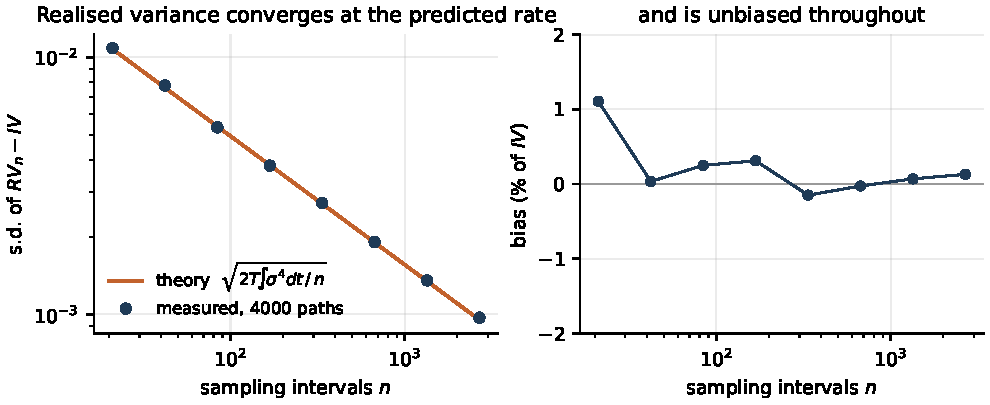
\includegraphics[width=0.52\linewidth]{figures/rv_convergence.pdf}
\caption{Left: dispersion of $RV_n-IV$ (points) against the closed form~\eqref{eq:rvse}
(line) --- a prediction, not a fit. Right: the estimator is unbiased throughout.}
\end{figure}

\section{Measurement: NIFTY volatility, and where GBM breaks}
\label{sec:measure}

Applying~\eqref{eq:rv} over rolling 21-day windows and annualising, realised volatility
averages $\mathbf{14.17\%}$ with standard deviation $8.08\%$ and a range of
$\mathbf{5.37\%}$ to $\mathbf{88.45\%}$ (the peak in March 2020). No constant $\sigma$
approximates a quantity moving over a sixteen-fold range, but the \emph{manner} of failure is
what matters and it is specific. \textbf{Clustering:} the autocorrelation of $|r_t|$ is
$+0.256$ at lag~1 and still $+0.080$ at lag~42, with Ljung--Box $Q(10)=1752.1$ on squared
returns against a $1\%$ critical value of $23.2$; volatility is overwhelmingly predictable from
its own past, where constant-$\sigma$ GBM implies zero autocorrelation at every lag.
\textbf{Returns are close to, but not exactly, unpredictable:} $Q(10)=59.3$ on the returns
themselves also exceeds $23.2$, driven mainly by lags 5 and 10. Return autocorrelation is small
but statistically detectable --- an order of magnitude weaker than the variance structure, not
zero. \textbf{Asymmetry:} $\operatorname{corr}(r_t,\Delta\hat\sigma_t)=-0.200$, so volatility
rises on down moves; GBM is symmetric in $W$ and cannot produce this, which is why the real
option surface carries a skew. \textbf{Vol-of-vol:} $99.2\%$ annualised --- an \emph{upper
bound}, since differencing a 21-day window daily injects measurement noise. No result depends
on it.

\section{Valuation: the market's forecast error, and what it is worth}
\label{sec:value}

\textbf{Unbiasedness.} Pairing the India VIX quoted at the start of each of 138
non-overlapping 21-day cycles with the realised volatility that followed, and regressing
realised on implied (Mincer--Zarnowitz),
\[
  \sr=a+b\,\si+\varepsilon,\qquad
  \hat a=0.0310\ (0.0163),\quad \hat b=0.6637\ (0.0909),\quad R^2=0.282 .
\]
Unbiasedness requires $a=0$, $b=1$; the slope is rejected, $t_{b=1}=-3.70$. Implied volatility
is informative --- it explains $28\%$ of the variation in what follows and $\hat b$ is $7.3$
standard errors from zero --- but it \textbf{overreacts}: a one-point rise in India VIX is
followed on average by only two-thirds of a point of extra realised volatility. The intercept
is positive but insignificant at $5\%$ ($t=+1.91$). Cycles are non-overlapping precisely so
these standard errors are not inflated by the serial correlation overlapping windows induce.

\textbf{The premium.} Mean implied volatility is $16.66\%$ against mean subsequent realised
volatility $14.16\%$: a gap of $\mathbf{+2.50}$ volatility points, positive in
$\mathbf{76.8\%}$ of the 138 months, $t=+4.04$. In variance terms $\E[\si^2-\sr^2]=+0.00531$.

\begin{figure}[tbp]
\centering
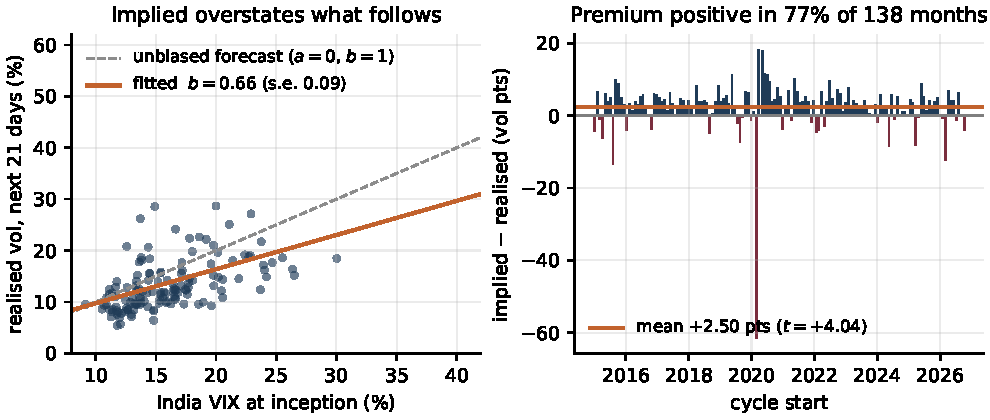
\includegraphics[width=0.52\linewidth]{figures/implied_vs_realised.pdf}
\caption{Left: realised against implied, with the unbiasedness line and the fitted line.
Right: the gap, month by month.}
\end{figure}

\textbf{What It\^o says the gap is worth.} The gap is tradeable, and It\^o's lemma says by how
much. Sell an option at $\si$ and delta-hedge at $\si$ while the index realises $\sigma_t$.
Applying It\^o to $V(S_t,t)$ along the realised path and substituting the Black--Scholes PDE
that $V(\cdot;\si)$ satisfies, the $\dd W$ terms cancel by construction of
$\Delta=\partial V/\partial S$, leaving the self-financing portfolio's terminal P\&L
\begin{equation}
  \Pi_T=\half\int_0^T e^{r(T-t)}S_t^2\,\Gamma_t\,\big(\si^2-\sigma_t^2\big)\,\dd t ,
  \label{eq:pnl}
\end{equation}
a \emph{pathwise} identity: the hedger is long the variance gap, weighted by dollar gamma.
Two results confirm it. \textbf{(i) The discretisation cost.} Continuous rebalancing is
unavailable; with $n$ rebalances the residual has standard deviation $\propto n^{-1/2}$
\cite{boyle1980}. On simulated GBM with $\sigma$ known the measured log--log slope is $-0.470$
across all settings, tightening monotonically to $\mathbf{-0.489}$ for $n\ge21$, with mean
error indistinguishable from zero: discrete hedging is unbiased, and it is the dispersion that
costs. \textbf{(ii) The identity on real paths.} Evaluating~\eqref{eq:pnl} along each realised
NIFTY path and comparing with the hedged position's actual P\&L --- computed independently by
a self-financing accounting simulation --- gives $\operatorname{corr}=\mathbf{+0.949}$
(predicted $+39.2$ points per cycle against actual $+36.1$). The trade earns $+36.06$ points
per cycle, $+11.31\%$ of premium, s.d.\ $88.30$, positive in $74.6\%$ of cycles, $t=4.80$
($p=4.1\times10^{-6}$), cumulating to $+4{,}977$ points.

\begin{figure}[tbp]
\centering
\begin{minipage}{0.435\linewidth}
  \centering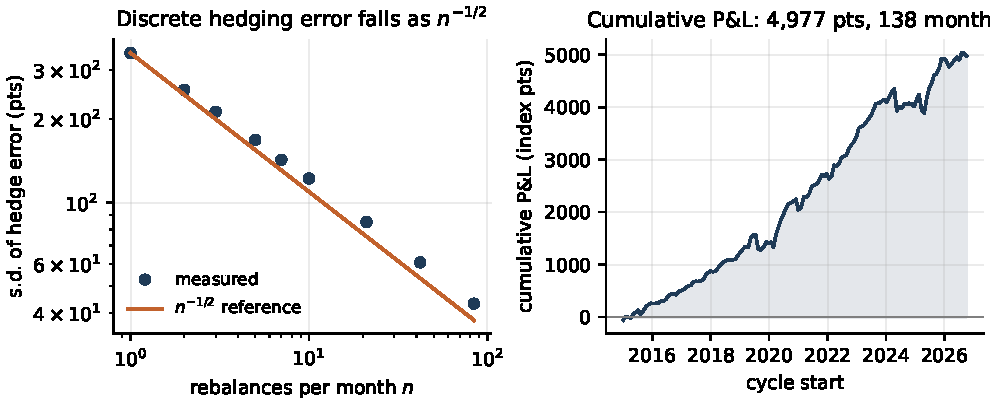
\includegraphics[width=\linewidth]{figures/hedge.pdf}
\end{minipage}\hfill
\begin{minipage}{0.22\linewidth}
  \centering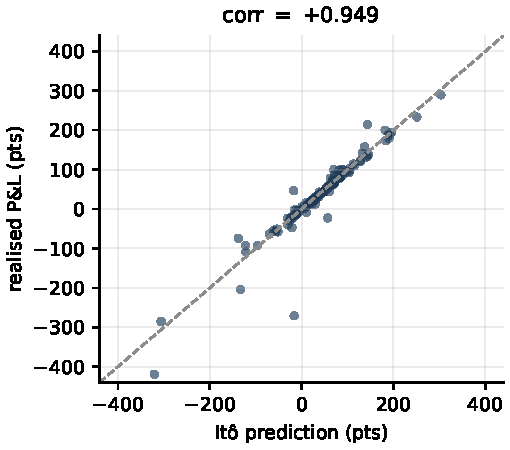
\includegraphics[width=\linewidth]{figures/ito_vs_actual.pdf}
\end{minipage}
\caption{Left: the $n^{-1/2}$ law, and cumulative P\&L of the hedged short call. Right:
equation~\eqref{eq:pnl} evaluated pathwise against realised P\&L, 138 cycles.}
\end{figure}

\begin{keybox}[Why the P\&L identity survives data the model does not describe]
NIFTY log returns have excess kurtosis $19.3$ and skew $-1.27$, and Section~\ref{sec:measure}
shows volatility is neither constant nor symmetric, so $r=0.949$ needs an explanation rather
than a celebration. It is this: \eqref{eq:pnl} is a \emph{pathwise} consequence of It\^o's
lemma, deriving only from $S$ being a continuous semimartingale with quadratic variation
$\int\sigma_t^2\dd t$ --- the object Section~\ref{sec:verify} verified. It never uses
normality, independence or constancy of $\sigma$. Fat tails and clustering change \emph{what}
$\int\sigma_t^2\dd t$ turns out to be; they do not break the identity relating it to P\&L.
\end{keybox}

\section{Robustness}
\label{sec:robust}

Three objections are answered by computation rather than by argument.

\textbf{Jumps.} Identity~\eqref{eq:qv} assumes a \emph{continuous} semimartingale; if the price
jumps, $RV_n$ converges to $\int\sigma_t^2\dd t+\sum(\text{jump})^2$. Bipower variation
$BV=\tfrac{\pi}{2}\sum|r_i||r_{i-1}|$ is jump-robust --- a lone large $|r_i|$ is multiplied by a
normal-sized neighbour --- and still estimates $\int\sigma_t^2\dd t$, so $RV-BV$ estimates the
jump part \cite{bns2004}. The full-sample jump share is $\mathbf{5.60\%}$ and the
Barndorff-Nielsen--Shephard ratio statistic is $Z=+1.617$, \textbf{short of the $5\%$ critical
value $1.96$}; year by year the no-jump null is rejected in only 2 of 12 years.
\textbf{About $94\%$ of NIFTY quadratic variation is diffusive}, so the continuity assumption
is empirically adequate here.

\textbf{Transaction costs.} A proportional cost on every rebalance separates two effects. At
zero cost the mean P\&L is \emph{not} a function of rebalance frequency --- spread $22.5$
points against a typical standard error of $11.9$ --- exactly as unbiasedness requires; what
frequency buys is dispersion, the standard deviation falling from $230$ points (two
rebalances) to $88$ (daily). The cost drag is deterministic and grows \textbf{sublinearly},
log--log slope $+0.30$ against trade count rather than $+1$, because rebalancing more often
makes each trade smaller. Hedging daily the premium survives at $+32.4$ points at $1$~bp
($t=4.30$), $+28.8$ at $2$~bps ($t=3.81$) and $+17.8$ at $5$~bps ($t=2.33$), breaking even
near $10$~bps. Indian index-futures round trips sit at the low end of that range, so
\textbf{the premium is not an artefact of ignoring costs}.

\textbf{Regime stability.} On disjoint sub-periods the result holds throughout:
$2015$--$2019$ gives $+24.0$ points per cycle ($t=3.22$), COVID $2020$--$2021$ gives $+56.9$
($t=2.91$), $2022$--$2026$ gives $+40.2$ ($t=2.74$) --- larger when volatility is higher, as a
risk premium should be.

\begin{figure}[tbp]
\centering
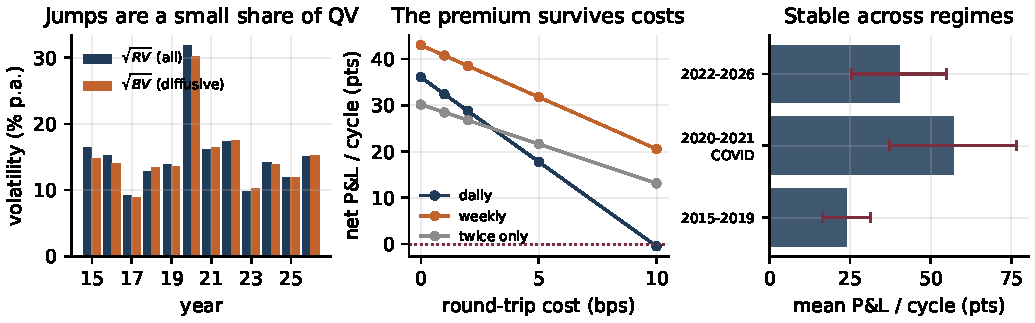
\includegraphics[width=0.60\linewidth]{figures/robustness.pdf}
\caption{Left: realised against jump-robust bipower volatility, by year. Centre: net P\&L
against transaction cost. Right: mean P\&L by sub-period, $\pm1$ standard error.}
\end{figure}

\section{Limitations}
\vspace{-0.15cm}
\begin{itemize}[leftmargin=*,topsep=0pt,itemsep=0.5pt]
  \item \textbf{The premium is reconstructed, not quoted.} Both inputs are market data ---
        NIFTY closes, and an India VIX built from traded NIFTY option prices --- but the option
        sold in Section~\ref{sec:value} is Black--Scholes at $\si$, not a quote from the chain
        at that strike and expiry. Section~\ref{sec:measure} and the forecast test use spot and
        VIX alone; what inherits the model is the \emph{level} of the backtest P\&L, not the
        variance gap driving it. A model-free $\si$ and an at-the-money strike bound the error;
        replicating this on the NSE chain, bid--ask included, would settle it.
  \item \textbf{Costs are modelled, not measured.} Section~\ref{sec:robust} applies a
        proportional cost; it omits margin funding and market impact. The premium survives
        plausible costs; that is not the claim that a desk would realise it net.
  \item \textbf{Daily closes only, and limited scope.} $RV_n$ at daily frequency is coarse;
        intraday data would sharpen it and the jump test, whose asymptotics are weak at
        $n\approx250$. Close-to-close sampling puts untradeable overnight gaps into $RV$. India
        VIX is a 30-calendar-day index on a 21-trading-day cycle --- a bias in the level of
        $\si$, not the sign of the gap. One index, at-the-money calls, flat $r$.
\end{itemize}

\section{Conclusion}

Volatility in the It\^o framework is a quadratic variation, and that is not a formality: it
makes volatility measurable from one path, gives the estimator a verifiable rate \emph{and}
constant, and supplies the pathwise identity~\eqref{eq:pnl} turning a forecast error into a
P\&L. The NIFTY~50 bears this out --- the estimator behaves as predicted, $94\%$ of the
quadratic variation is diffusive, the index violates constant-$\sigma$ GBM through clustering
and asymmetry rather than at random, India VIX overreacts with slope $0.66$, and the resulting
premium is recovered at correlation $0.949$ with what It\^o predicts and survives realistic
costs. A model can be wrong about the distribution of returns and still be exactly right about
the accounting.

\paragraph{Reproducibility.} Six flat modules (\texttt{sc\_data}, \texttt{sc\_model},
\texttt{sc\_vol}, \texttt{sc\_hedge}, \texttt{sc\_robust}, \texttt{sc\_figures}) with a fixed
seed. Before any result is computed the model layer verifies the PDE residual to
$3.4\times10^{-6}$ relative, Greeks against finite differences to $10^{-8}$, and put--call
parity to six decimals.

\vspace{-0.1cm}
\begin{multicols}{2}\scriptsize
\begin{thebibliography}{9}
\scriptsize
\setlength{\itemsep}{-1pt}
\bibitem{boyle1980} Boyle, P.\,P.\ and Emanuel, D. (1980). Discretely adjusted option hedges.
  \emph{J.\ Financial Economics} \textbf{8}(3), 259--282.
\bibitem{bs1973} Black, F.\ and Scholes, M. (1973). The pricing of options and corporate
  liabilities. \emph{J.\ Political Economy} \textbf{81}(3), 637--654.
\bibitem{shreve2004} Shreve, S.\,E. (2004). \emph{Stochastic Calculus for Finance II}. Springer.
\bibitem{bn2002} Barndorff-Nielsen, O.\,E.\ and Shephard, N. (2002). Econometric analysis of
  realised volatility. \emph{JRSS\ B} \textbf{64}(2), 253--280.
\bibitem{cw2009} Carr, P.\ and Wu, L. (2009). Variance risk premiums. \emph{Rev.\ Financial
  Studies} \textbf{22}(3), 1311--1341.
\bibitem{mz1969} Mincer, J.\ and Zarnowitz, V. (1969). The evaluation of economic forecasts.
  In \emph{Economic Forecasts and Expectations}. NBER.
\bibitem{bns2004} Barndorff-Nielsen, O.\,E.\ and Shephard, N. (2004). Power and bipower
  variation with stochastic volatility and jumps. \emph{J.\ Financial Econometrics}
  \textbf{2}(1), 1--37.
\bibitem{ht2005} Huang, X.\ and Tauchen, G. (2005). The relative contribution of jumps to total
  price variance. \emph{J.\ Financial Econometrics} \textbf{3}(4), 456--499.
\end{thebibliography}
\end{multicols}

\end{document}
